\documentclass[a4paper,11pt,fleqn]{article}%fleqn pour aligner les equations à gauche
\usepackage{../../Styles/Exercice}


\newcommand{\chnum}{Chapitre 02}
\newcommand{\chtitle}{Couleur des objets}
\newcommand{\dtype}{Exercices}
  
\begin{document}

\maketitle

\begin{multicols}{2}
\section{Impression couleur}
\begin{minipage}
    {.6\linewidth}
    Sur un papier blanc, on souhaite imprimer une image de Marge Simpson : sa peau jaune, son collier rouge, son tailleur vert et les traits de dessin noir.
\begin{enumerate}
    \item Quel type de synthèse est mis en \oe uvre dans une imprimante ?
    \item Dessiner le cercle chromatique correspondant.
    \item Donner les superpositions d'encres à faire pour obtenir la couleur souhaitée de Marge.
\end{enumerate}
\end{minipage}
\begin{minipage}{.35\linewidth}
    \begin{center}
        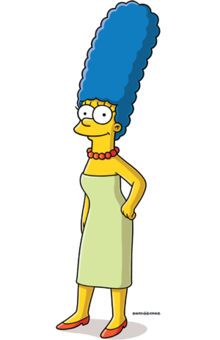
\includegraphics[width=\linewidth]{Ressources/Marge.png}
    \end{center}
\end{minipage}

\section{Défaut d'éclairage}
Une scène est éclairée par trois projecteurs correspondant chacun à une couleur primaire. Un projecteur tombe en panne et un acteur habillé de blanc apparaît alors magenta aux yeaux des spectateurs.
\begin{enumerate}
    \item Quelles sont les trois couleurs des projecteurs de la scène ?
    \item Quel est le projecteur qui est tombé en panne ?
\end{enumerate}

\section{Association de filtres colorés}
On dispose de trois projecteurs de lumière rouge, verte et bleue et de trois filtres de couleurs primaires en synthèse soustractive (cyan, magenta et jaune).
\begin{enumerate}
    \item Comment obtenir une lumière cyan à l'aide des projecteurs ?
    \item Que ressort-il d'un filtre cyan éclairé par une lumière cyan ?
    \item On rajoute derrière ce filtre cyan un filtre jaune. Quelle couleur ressort ?
\end{enumerate}

\section{Drapeaux}
Lors du match France-Allemagne, les drapeaux des pays sont projetés sur un écran géant. Les lumières arrivent sur un spectateur qui porte des lunettes un peu spéciales.\\
\begin{center}
    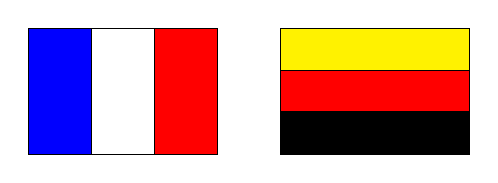
\begin{tikzpicture}[scale=0.8]
        % Drapeau France
        \draw[fill=blue] (0,0) rectangle (1,2);
        \draw[fill=white] (1,0) rectangle (2,2);
        \draw[fill=red] (2,0) rectangle (3,2);
        % Drapeau Allemagne
        \draw[fill=black] (4,0) rectangle (7,0.67);
        \draw[fill=red] (4,0.67) rectangle (7,1.33);
        \draw[fill=yellow] (4,1.33) rectangle (7,2);
    \end{tikzpicture}
\end{center}
Le premier spectateur a des verres cyan.
\begin{enumerate}
    \item Quel est le type de synthèse mis en jeu dans cette situation ?
    \item Établie le schéma correspndant.
    \item Quelles(s) est/sont la/les couleur(s) absorbée(s) par le filtre cyan ?
    \item En déduire les lumières transmises.
    \item Conclure en dessinant les couleurs des drapeaux vues par le spectateur.
\end{enumerate}

Le deuxième spectateur a un verre gauche vert et un verre droit rouge.
\begin{enumerate}
    \item Quel est le sytpe de synthèse mis en jeu ?
    \item Quelle(s) est/sont la/les couleur(s) absorbée(s) par le filtre vert ? et par le filtre rouge ?
    \item Conclure en dessinant les couleurs des drapeaux vues par le spectateur par son \oe il gauche et par son \oe il droit.
\end{enumerate}
Le troisième spectateur a un verre gauche magenta et un verre droit bleu.
\begin{enumerate}
    \item En argumentant et en justifiant, dessiner ce que voit le spectateur en fermant l'\oe il gauche puis en fermant l'\oe il droit.
\end{enumerate}
\end{multicols}
\end{document}
